\section{Generalisation und Regularisierung}
\subsection{Overfitting}
Overfitting ist wenn alle Punkte genau getroffen werden. Dann stimmt es zwar für die Trainingsdaten genau, aber sobald weiter Datenpunkte dazukommen stimmt es für diese nicht mehr. Wir haben zwar einen MSE von 0, dies ist aber ein \textbf{In-Sample Error (Training Error)}. Der Loss wurde sehr stark minifiziert in der Trainingsphase.\\
\\
Sobald wir dann aber die Testdaten dazu nehmen (Neue noch nicht gesehene Daten, haben wir dann einen grossen \textbf{Out Of
Sample Error (Generalization Error)}. Ein gutes Modell hat ein tiefen Generalization Error.\\
\\
Ziel: tieferer Generalization Error, In-Sample Error darf aber grösser sein
\subsection{Underfitting}
Underfitting tritt dann auf, wenn das Modell zu einfach ist. Wir haben ein viel zu hoher In Sample Error, als auch ein zu grosser Generalization Error. Ein Beispiel dafür wäre eine Gerade, welche durch ein sehr komplexes Model durchgeht und sehr viel verpasst. Gegenteil von Overfitting.
\subsection{Generalization Error}
Der Generalization Error kann nicht berechnet werden, sondern nur geschätzt werden. Wir müssen mit den Daten arbeiten, die wir haben. Deshalb müssen wir unsere Daten splitten in Test- und Trainingsdaten. Ein guter Split ist 80\% Training und 20\% Test. So nutzt man die Training-Daten um das Modell zu trainieren und wenden dann mit den Testdaten das Modell an. Der Test-Fehler ist eine Schätzung vom Generalization Fehler.
\subsection{Bias und Varianz}
Wenn wir die beiden Fehler genauer mathematisch analysieren können wir zwei Werte feststellen: Bias und Varianz.\\
\textcolor{myblue}{High Bias, Low Variance}\\
In diesem Fall ist das Modell zu einfach. Egal wie viele Daten wir haben, das Modell gibt keine besseren Ergebnisse. Zum Beispiel wir nehmen ein Lineares Modell obwohl es passendere gibt. Dann ist dieses zu einschränkend. Die rote Linie wird bei vielen Daten gleich bleiben auch wenn ich ein neuer Punkt hinzufüge. Wir haben underfitting.\\
\textcolor{myblue}{Low Bias, High Variance}\\
Man nimmt ein (zu) komplexes Modell. Es kann die Daten besser beschreiben. Beispiel 6 Punkte und wir nehmen ein Polynom Grad 5. Hier passt das Modell genau zu den Testdaten. Aber wir haben nun Overfitting.Die Varianz ist hoch. Ein weiter Datenpunkt führt dann zu einem sehr grossen Generalization error. Und sobald ein Punkt etwas verschoben ist, ist die Line komplett eine andere.
\subsection{Regularisierung}
Unser Ziel: Wir wollen möglichst eine tiefe Varianz. Der Bias ist eher sekundär, sollte aber auch möglichst tief sein. Man braucht aber die optimale Balance. Am besten schauen wir da den Training- und Testerror genauer an. Es gibt einen Punkt wo der Testerror am tiefsten ist und dann wieder steigt je genauer das Modell ist. Dazu verwenden wir Regularisierung.
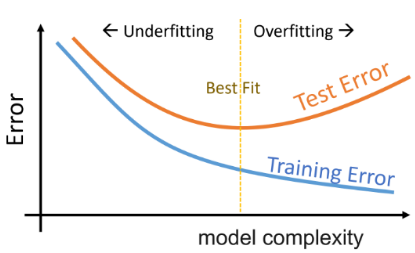
\includegraphics[width=\linewidth]{img/regularization.png}
Regularisierung fügt Constrains hinzu, ein Penalty-Term (Cost-Function). Der Optimizer optimiert die Daten (MSE minimalisieren) sowie auch den Constraint.
Es gibt zwei Zutaten die wir benötigen:
\begin{enumerate}
\item Weg zum Modell-Komplexität zu messen
\begin{itemize}
\item L1 Norm (Lasso) 
$$\sum_{j=1}^p | \beta_j|$$
\item L2 Norm (Ridge)
$$\sum_{j=1}^p \beta^2_j$$
\end{itemize}
\item Weg zum Model-Komplexität zu kontrollieren
\begin{itemize}
\item Penalty-Term wird zu Loss hinzugefügt
\item Komplexere Modelle haben höhere Penalty
\item Constraint wird zum Optimierungsprozess hinzugefügt
$$\sum_{i=1}^n(y_i-\sum_{j=1}^p x_{ij} \beta_j)^2+ \lambda \sum_{j=1}^p \beta^2_j$$
\end{itemize}
\end{enumerate}

«Lamda ist der Hyperparameter»\\
Lamda = 0: dann haben wir kein Constraint also nur MSE. Vergrössern von Lamda: zu grosse Bias, kleinere Varianz\\
\textbf{Beispiel}: Wenn man zwei Modelle gegeben hat, die mit verschiedenen Regulasierungswerten($\lambda$) trainiert wurden, dann wähle das Modell, das im Schnitt die besseren Werte erzielt. Bei grösseren Regulasierungswerten ($\lambda$) erhält man tiefere Varianz, aber höheres Bias. Doch bei einer grossen Varianz soll man ein neues Modell trainieren, mit dem Besseren Regularisierungswert($\lambda$).
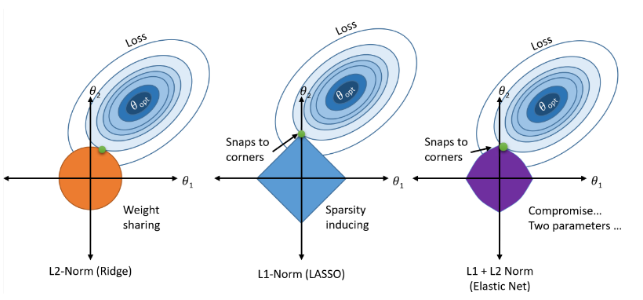
\includegraphics[width=\linewidth]{img/l-norm.png}